% !TEX TS-program = xelatex
% !TEX encoding = UTF-8

\documentclass[12pt]{book} % use larger type; default would be 10pt

\usepackage{amssymb}
\usepackage{fontspec} % Font selection for XeLaTeX; see fontspec.pdf for documentation
%\defaultfontfeatures{Mapping=tex-text} % to support TeX conventions like ``---''
%\usepackage{xunicode} % Unicode support for LaTeX character names (accents, European chars, etc)
%\usepackage{xltxtra} % Extra customizations for XeLaTeX

\setmainfont[Numbers=OldStyle]{CJunicode} % set the main body font (\textrm), assumes Charis SIL is installed
%\setsansfont{Deja Vu Sans}
%\setmonofont{Deja Vu Mono}

\usepackage{scalefnt}
\newcommand{\mathipa}[1]{\textrm{\scalefont{1.08}\selectfont #1}} % scaled to 1.1 also seems ok


% other LaTeX packages.....
\usepackage{geometry}
\geometry{letterpaper} % or a4paper (US) or a5paper or....
%\usepackage[parfill]{parskip} % Activate to begin paragraphs with an empty line rather than an indent

\usepackage{multicol}

\usepackage{float}
\usepackage{subcaption}
\usepackage{rotating}

\usepackage{graphicx} % support the \includegraphics command and options
\usepackage{tikz}

\usepackage{xcolor}
\usepackage{colortbl}
\definecolor{Gray}{gray}{0.9}
\newcolumntype{a}{>{\columncolor{Gray}}c}


\usepackage{qtree}
\usepackage{mathtools}





\title{Utsišcy /ˈutsiʃkɨ/ \\ {\Large Draft Grammar}}
\author{Okuno Zankoku}
%\date{} % Activate to display a given date or no date (if empty),
         % otherwise the current date is printed 

\begin{document}
\maketitle





\chapter{Demography and Ethnography}
So, what is this language, Utsišcy?

It's certainly an art language, as its only purpose is my enjoyment and hopefully someone else's as well.
If I describe it as a naturalistic language, that's because I think the assymmetries of natural languages are aesthetically pleasing in a wabi-sabi sort of way.
I've spared little thought for relative infrequencies of the various features I've chosen to include in preference to what I find fun, as long as the result is ``harmonious''.

Many naturalistic artlangs are also embedded in a conworld and come with a conculture, but that's not what I'm really interested in.
This language has no conceit (as fun as they can be); it is made up by a single person, and I present it that way.
I sometimes mention Utsišcy's ``history'' (which it doesn't have), it is only to allow me to explore the relation of some twist to the rest of the language and understand how to balance it.

At the end of the day, I'm not even sure I'm conlanging: I think I'm con-ideolecting.


FIXME: tʃ' needs to look more like tʃ\,'


\chapter{Sound System}

\section{Phonemics}

The number of phonemes available in Utsišcy varies depending on your theoretical predelictions.
There are several clusters analyzable as affricates and most consonants may be labialized or palatalized, which quite explodes the count of consonants.
The perspective I take is that apparently affricate, labialized, and palatalized consonants are underlyingly clusters.
This gives 43 phonemes, a large inventory even at this conservative analysis.

\begin{figure}[H]
\centering
\begin{subtable}[t]{0.5\linewidth}
	\centering
	\begin{tabular}{ccccc}
		\hskip 0.7em m & \hskip 0.8em n \\
		p b & t d & c ɟ & k \\
		\hskip 0.8em ɓ & t' ɗ & c' ʄ & k' \\
		f v & s z & ʃ ʒ & x \\
		& \hskip 0.8em s' & \hskip 0.8em ʃ' & x' \\
		& r̥ r & & & ʀ \\
		& l̥ l & ʎ̥ ʎ \\
		 && j̊ j \\
	\end{tabular}
	\caption{consonants}\label{t:phoneme-consonants}
\end{subtable}
\hskip -6em
\begin{subtable}[t]{0.5\linewidth}
	\centering
	\begin{tabular}{cc}
		i & ɨ u \\
		ɛ & a ɔ \\
		◌ʲ & \; ◌ʷ\\
	\end{tabular}
	\caption{vowels}\label{t:phoneme-vowels}
\end{subtable}
\caption{Phoneme Intentory}\label{t:phonemes}
\end{figure}

Several consistently distinctive features support the inventory size.
First, stops have four voicings in most places: unvoiced, voiced, ejective, and implosive; the only exceptions are the cross-linguistically common gaps /p', g, ɠ/.
Likewise, fricatives have three voicings in most places: unvoiced, voiced, and ejective.
The presence of ejective fricatives is unusual, but again the gaps /f', ɣ/ are common.

Second, there is a distinction between palatals and velars.
Historically, this was a distinction between velar and uvular consonants which underwent fronting.
This brings some sanity to the appearance of a /ʄ/ < */k'/ phoneme without a corresponding */k'/ < **/q'/.

Third, Utsišcy consistently distinguishes between voiced and unvoiced variants of liquids /r̥, l̥, ʎ̥, j̊/ vs. /r, l, ʎ, j/.
Note that the two semi-vowel phonemes /◌ʷ, ◌ʲ/ are not considered liquid.
Nevertheless, they only appear bound to another phoneme, and in that capacity, they take on the voice of whatever consonant to which they attach.

A careful reader may note the presence of three trills, but it should be noted that only /r̥,~r/ pattern as rhotics in the lexicon; /ʀ/ < */ʁ/, and so patterns as a voiced fricative (TODO and probably also has [ʁ] as an allophone).

In comparison to the consonants, the vowel system is reserved.
It is similar to the Russian vowel system: a simple /i, e, a, o, u/ with a center-high vowel /ɨ/.

\subsection{Featural Analysis}

This section describes the precise phonetic features Utsišcy considers contrastive.
A summary table of features for each phoneme is given in fig.\ \ref{fig:phoneme-features}; phonological processes in the sequent refer there.
A reader uninterested in the finer theoretical points may otherwise skip fearlessly to \S\ref{sec:orthography}.

\subsubsection{Feature Inventory}

I'm sticking to fairly standard feature nomenclature.
One thing to be wary of is that palatal and velar places are not distinguished directly as part of the place category; instead, they are both [+dorsal], but palatal is [+front] and velar is not.

Just to help the reader avoid guesswork, I'll quickly review the feature abbreviations ($=$), synonyms ($\Leftrightarrow$) and antonyms ($\nLeftrightarrow$).
\begin{multicols}{2}
\begin{itemize}
\item $\mathipa{cons} = \mathipa{consonantal} \nLeftrightarrow \mathipa{vocoid}$
\item $\mathipa{vowel} \Leftrightarrow \mathipa{sonorant} \land \mathipa{vocoid}$
\item $\mathipa{glide} \Leftrightarrow \mathipa{obstruent} \land \mathipa{vocoid}$
\item $\mathipa{obs} = \mathipa{obstruent} \nLeftrightarrow \mathipa{sonorant} = \mathipa{son}$
\item $\mathipa{cg} = \mathipa{constricted glottis}$
\item $\mathipa{cont} = \mathipa{continuant}$
\item $\mathipa{back} \nLeftrightarrow \mathipa{front}$
\item $\mathipa{low} \nLeftrightarrow \mathipa{raised}$
\item $\mathipa{palatal} \Leftrightarrow \mathipa{front} \land \mathipa{dorsal}$
\end{itemize}
\end{multicols}

A table of phonemically-relevant features for each phoneme is given in fig. \ref{fig:phoneme-features}.
I've decided that /ʀ/ is phonemically a trill rather than a fricative, even though it was historically fricative.

\begin{sidewaysfigure}
\setlength\tabcolsep{2pt}
\begin{tabular}{r ccaaa cccca  aaacc aaccc aaacc aaacc  aacca aaaaa  cc}
&
m & n &
p & b & ɓ & t & d & t' & ɗ & c & ɟ & c' & ʄ & k & k' &
f & v & s & z & s' & ʃ & ʒ & ʃ' & x & x' &
r̥ & r & ʀ &
l̥ & l & ʎ̥ & ʎ & j̊ & j &
i & ɨ & u &
ɛ & a & ɔ &
◌ʷ & ◌ʲ \\

% && &&& &&&& &&&& && && &&& &&& && &&& && && && &&&&&& && \\

\multicolumn{1}{l}{\textbf{Major}} \\
%syllabic && &&& &&&& &&&& && && &&& &&& && &&& && && && &&&&&& && \\
consonantal &+&+ &+&+&+ &+&+&+&+ &+&+&+&+ &+&+ &+&+ &+&+&+ &+&+&+ &+&+ &+&+&+ &+&+ &+&+ &+&+ &-&-&-&-&-&- &-&- \\
%approximant && &&& &&&& &&&& && && &&& &&& && &&& && && && &&&&&& && \\
sonorant &+&+ &-&-&- &-&-&-&- &-&-&-&- &-&- &-&- &-&-&- &-&-&- &-&- &+&+&+ &+&+ &+&+ &+&+ &+&+&+&+&+&+ &-&- \\

\multicolumn{1}{l}{\textbf{Laryngeal}} \\
voice && &-&+& &-&+&& &-&+&& && &-&+ &-&+& &-&+& &-& &-&+& &-&+ &-&+ &-&+ &&&&&& && \\
%spread glottis && &&& &&&& &&&& && && &&& &&& && &&& && && && &&&&&& && \\
\qquad
constricted glottis && &-&-&+ &-&-&+&+ &-&-&+&+ &-&+ &-&- &-&-&+ &-&-&+ &-&+ &&& && && && &&&&&& && \\

\multicolumn{1}{l}{\textbf{Manner}} \\
explosive && &&&- &&&+&- &&&+&- &&+ && &&& &&& && &&& && && && &&&&&& && \\
continuant && &-&-&- &-&-&-&- &-&-&-&- &-&- &+&+ &+&+&+ &+&+&+ &+&+ &&& && && && &&&&&& && \\
nasal &+&+ &&& &&&& &&&& && && &&& &&& && &-&-&- &-&- &-&- &-&- &&&&&& && \\
%strident && &&& &&&& &&&& && && &&& &&& && &&& && && && &&&&&& && \\
vibrant &-&- &&& &&&& &&&& && && &&& &&& && &+&+&+ &-&- &-&- &-&- &&&&&& && \\
lateral &-&- &&& &&&& &&&& && && &&& &&& && &-&-&- &+&+ &+&+ &-&- &&&&&& && \\

\multicolumn{1}{l}{\textbf{Place}} \\
labial &+&- &+&+&+ &-&-&-&- &-&-&-&- &-&- &+&+ &-&-&- &-&-&- &-&- &&& && && && &&&&&& &+&- \\
coronal &-&+ &-&-&- &+&+&+&+ &-&-&-&- &-&- &-&- &+&+&+ &-&-&- &-&- &&& && && && &&&&&& && \\
dorsal &-&- &-&-&- &-&-&-&- &+&+&+&+ &+&+ &-&- &-&-&- &+&+&+ &+&+ &-&-&+ &-&- &+&+ && &&&&&& && \\
%pharyngeal && &&& &&&& &&&& && && &&& &&& && &&& && && && &&&&&& && \\
%glottal && &&& &&&& &&&& && && &&& &&& && &&& && && && &&&&&& && \\

\multicolumn{1}{l}{\textbf{Tongue Posture}} \\
front && &&& &&&& &+&+&+&+ &-&- && &&& &+&+&+ &-&- &&& && && && &+&-&-&+&-&- && \\
%retracted && &&& &&&& &&&& && && &&& &&& && &&& && && && &&&&&& && \\
raised && &&& &&&& &&&& && && &&& &&& && &&& && && && &+&+&+&-&-&- && \\
round && &&& &&&& &&&& && && &&& &&& && &&& && && && &&-&+&&-&+ && \\
%tense/atr && &&& &&&& &&&& && && &&& &&& && &&& && && && &&&&&& && \\
%rtr && &&& &&&& &&&& && && &&& &&& && &&& && && && &&&&&& && \\
\end{tabular}
\caption{Phoneme Features}\label{fig:phoneme-features}
\end{sidewaysfigure}


\subsubsection{Contrastive Hierarchy}

Given that Utsišcy have very many phonemes, I've split the hierarchy into figs.\ \ref{fig:contrast-hier-top}--\ref{fig:contrast-hier-continuants}.
The hierarchy begins in fig.\ \ref{fig:contrast-hier-top}, which then will direct you to the figures for subhierarchies.
`Marked' values consistently branch to the left.

While I was building Utsišcy's contrastive hierarchy, I noticed that the ordering of some feature pairs seemed irrelevant.
I therefore decided to experiment with a description in terms of a partial-ordering rather than the more familiar total ordering.
The result is given in fig.\ \ref{fig:hier-summary}, and seems to be a useful, if incomplete, summary view of the hierarchy.
When feature $\alpha$ is connected to a lower feature $\beta$, then $\alpha > \beta$ in the hierarchy, and whether $\beta$ is contrastive is conditioned by the choice of $\alpha$.
For a full understanding of how features condition the others, consult the full hierarchy (figs.\ \ref{fig:contrast-hier-top}--\ref{fig:contrast-hier-continuants}).



\begin{figure}[H]
\centering
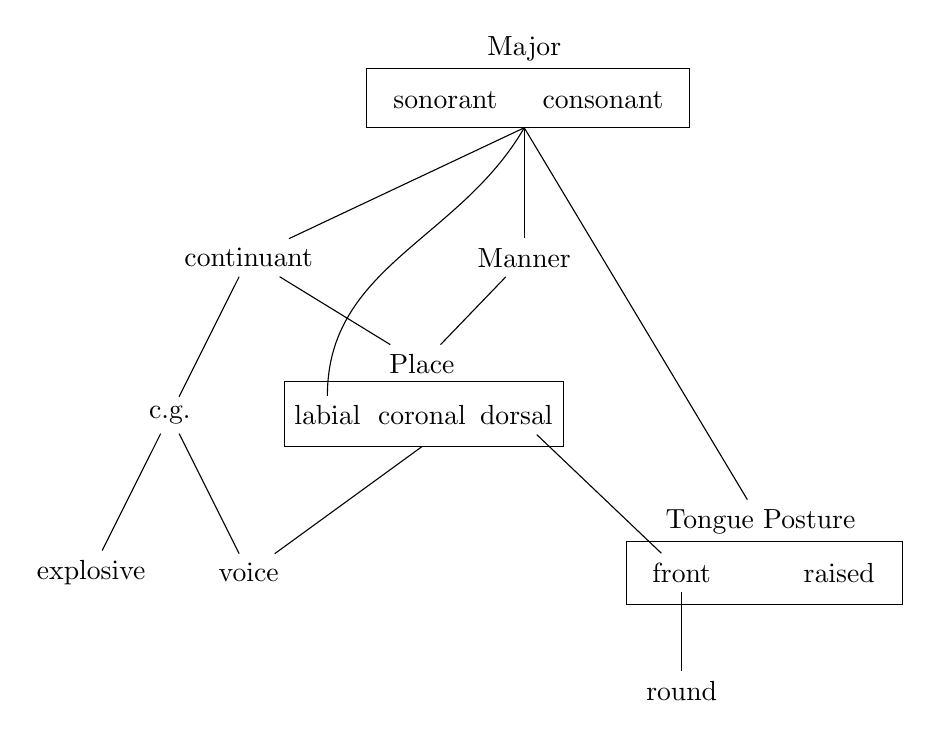
\begin{tikzpicture}
\node at (0,10.65) {Major};
\node (sonorant) at (-1, 10) {sonorant};
\node (consonant) at (1,10) {consonant};
\draw (-2,10.4) rectangle (2.1,9.65);
\coordinate (Major-out) at (0,9.65);

\node (continuant) at (-3.5,8) {continuant};
\draw (Major-out) -- (continuant);

\node (Manner) at (0,8) {Manner};
\draw (Major-out) -- (Manner);

\node (cg) at (-4.5,6) {c.g.};
\draw (continuant) -- (cg);

\node (Place) at (-1.3,6.65) {Place};
\node (labial) at (-2.5,6) {labial};
\node (coronal) at (-1.3,6) {coronal};
\node (dorsal) at (-0.1,6) {dorsal};
\draw (-3.05,6.43) rectangle (0.5,5.6);
\coordinate (Place-out) at (-1.3,5.6);
\draw (continuant) -- (Place);
\draw (Manner) -- (Place);
\draw [out=-120,in=90] (Major-out) to (labial);

\node (explosive) at (-5.5,4) {explosive};
\draw (cg) -- (explosive);

\node (voice) at (-3.5,4) {voice};
\draw (cg) -- (voice);
\draw (Place-out) -- (voice);

\node (Tongue) at (3,4.65) {Tongue Posture};
\node (front) at (2,4) {front};
\node (raised) at (4,4) {raised};
\draw (1.3,4.4) rectangle (4.8,3.6);
\draw (Major-out) to (Tongue);
\draw (dorsal) to (front);

\node (round) at (2,2.5) {round};
\draw (front) -- (round);
\end{tikzpicture}
\caption{Contrastive Hierarchy Summary}\label{fig:hier-summary}
\end{figure}



TODO Is it the case that the highest stuff has rules that allow/disallow, the lowest stuff has rules that assimilate, and the middle stuff retains its basic phonetics the best?
I'm pretty sure I'm doing voice assimilation, but not nasal assimilation or place assimilation for nasals, and that would be ``explained''.


\begin{figure}
\centering
\Tree [
	[.+consonantal
		\qroof{Liquids \\ \small fig.\ \ref{fig:contrast-hier-sonorants}}.+sonorant
		[.-sonorant
			\qroof{Fricatives \\ \small fig.\ \ref{fig:contrast-hier-continuants}}.+continuant
			\qroof{Stops \\ \small fig.\ \ref{fig:contrast-hier-stops}}.-continuant
		]
	]
	[.-consonantal
		[.-sonorant
			[.{\footnotesize +labial} ◌ʷ ]
			[.{\footnotesize -labial} ◌ʲ ]
		]
		\qroof{Vowels \\ \small fig.\ \ref{fig:contrast-hier-vowels}}.+sonorant
	]
]
\caption{Contrastive Hierarchy}\label{fig:contrast-hier-top}
\end{figure}

Even a cursory inspection of the top level of the hierarchy shows that the inventory is light on vowels and heavy on non-sonorant consonants.
Note that the non-sonorant vowels /◌ʷ, ◌ʲ/ appear here; as they are a small category, their ink on the page is easily overlooked.
Although the contraints of the tree have forced me to imply one of \{consonant,~vowel\} is marked, it's not entirely clear which should be.
%Since the [sonorant] is natural for vowels, but marked for consonants, we've used both [sonorant] and [obstruent] features, but these are simple antonyms of each other.

\begin{figure}
\centering
\Tree [.{-consonantal, +sonorant}
	[.{\footnotesize +raised}
		[.{\footnotesize -front}
			[.{\scriptsize +round} u ]
			[.{\scriptsize -round} ɨ ]
		]
		[.{\footnotesize +front} i ]
	]
	[.{\footnotesize -raised}
		[.{\footnotesize -front}
			[.{\scriptsize +round} ɔ ]
			[.{\scriptsize -round} a ]
		]
		[.{\footnotesize +front} ɛ ]
	]
]
\caption{Contrasive Hierarchy: vowels}\label{fig:contrast-hier-vowels}
\end{figure}

As suggested by fig. \ref{t:phoneme-vowels}, vowels are organized into a 2$\times$2 space with an additional rounding contrast only in the back vowels.
Although it is not clear from phonological processes, tongue posture sugggests [raised, back] are marked.\footnote{FIXME: Is this actually a thing? My guess is that there hasn't been enough research into the intersection of contrastive hierarchy and mouth posture to say; annoyingly, I don't think there's much research into mouth posture at all, except to inform accent training.}
Though I've had to decide on an order to draw the tree, given the symmetry between the two features it is likely that [raised] $\sim$ [front] rather than one taking a higher spot than the other.

\begin{figure}
\centering
\Tree [.{+consonantal, -sonorant, -continuant} 
	[
		[.{\footnotesize =labial}
			[ [ ɓ ] [ ◌ ] ]
			[ [ b ] [ p ] ]
		]
		[.{\footnotesize =dorsal}
			[.{\footnotesize -front}
				[ [ ◌ ] [ k' ] ]
				[ k ]
			]
			[.{\footnotesize +front}
				[ [ ʄ ] [ c' ] ]
				[ [ ɟ ] [ c ] ]
			]
		]
	]
	[.{\footnotesize =coronal}
		[.{\footnotesize +gc}
			[.{\footnotesize -explosive} ɗ ]
			[.{\footnotesize +explosive} t' ]
		]
		[.{\footnotesize -gc}
			[.{\footnotesize +voice} d ]
			[.{\footnotesize -voice} t ]
		]
	]
]
\caption{Contrastive Hierarchy: stops}\label{fig:contrast-hier-stops}
\end{figure}

In the stops (fig.\ \ref{fig:contrast-hier-stops}), I've elided many of the featural labels due to the number of phonemes.
The coronals have all the labels explicitly given; this pattern is implicitly replicated in the labials, velars, and palatals.
Some possible phonemes (*/p',~ɠ/) have been given as ``◌'' (empty): these do not appear in native words, but are never allophones of other phonemes.
Presumably these unattested phonemes could appear in loanwords\footnote{but where is Utsišcy going to borrow */p', ɠ/ from?}.
One exception to the pattern occurs in the velars [-front, =dorsal].
Although a voicing difference is to be expected between /k/ and */ɡ/, it does not occur.
I can't postulate an empty space here because /k/ is commonly realized as [ɡ].

An unfamiliar part of my analysis is that the implosives (/ɓ,~ɗ,~ɟ/) are [-continuant, -explosive] or, using more familiar names, [+stop, -obstruent].
I'm following Clements' paper ``Explosives, Implosives, and Nonexplosives: the Linguistic Function of Air Pressure Differences in Stops''.
There he uses [+stop, -obstruent] notation, which is apparently contradictory, but given his definition of obstruence (positive air pressure), technically makes sense.
I've opted to use the term [explosive], which is in keeping with Clement's more accessible prose (esp. the title and abstract, which use ``non-explosive'' repeatedly).

\begin{figure}
\centering
\Tree [.{+consonantal, -sonorant, +continuant}
	[
		[.{\footnotesize =labial}
			[ ◌ ]
			[ [ v ] [ f ] ]
		]
		[.{\footnotesize =dorsal}
			[.{\footnotesize -front}
				[ x' ]
				[ [ (ʀ) ] [ x ] ]
			]
			[.{\footnotesize +front}
				[ ʃ' ]
				[ [ ʒ ] [ ʃ ] ]
			]
		]
	]
	[.{\footnotesize =coronal}
		[.{\footnotesize +gc} s' ]
		[.{\footnotesize -gc}
			[.{\footnotesize +voice} z ]
			[.{\footnotesize -voice} s ]
		]
	]
]
\caption{Contrastive Hierarchy: fricatives}\label{fig:contrast-hier-continuants}
\end{figure}

The fricatives (fig.\ \ref{fig:contrast-hier-continuants}) have nearly the same structure as the stops.
The points of articulation are the same, and the only difference in the phonation is that [gc] fricatives do not distinguish an [explosive].
Again, there are too many phonemes to be fully explicit with feature labels, so the coronals are the only fricatives fully labelled.
There is one more phonemic gap (*/f'/) which behaves the same as the gaps in the stops.
Even though it is phonemically not a fricative, /ʀ/ was historically a fricative, and still occupies that phonetic space, so in loan words */ɣ,~ʁ/ > /ʀ/.

I've ordered place of articulation features higher in the hierarchy than phonation features because phonological rules are more likely to assimilate phonation rather than place.


\begin{figure}
\centering
\Tree [.{+consonantal, +sonorant}
			[.{\footnotesize +nasal}
				[.{\footnotesize +labial} m ]
				[.{\footnotesize -labial} n ]
			] !\qsetw{2cm}
			[.{\footnotesize -nasal}
				[.{\footnotesize +vibrant}
					[.{\scriptsize +dorsal} ʀ ]
					[.{\scriptsize -dorsal}
						[.{\scriptsize -voice} r̥ ]
						[.{\scriptsize +voice} r ]
					]
				]
				[.{\footnotesize -vibrant}
					[.{\footnotesize +lateral}
						[.{\footnotesize +dorsal}
							[.{\scriptsize -voice} ʎ̥ ]
							[.{\scriptsize +voice} ʎ ]
						]
						[.{\footnotesize -dorsal}
							[.{\scriptsize -voice} l̥ ]
							[.{\scriptsize +voice} l ]
						]
					]
					[.{\footnotesize -lateral}
						[.{\scriptsize -voice} j̊ ]
						[.{\scriptsize +voice} j ]
					]
				]
			]
		]
\caption{Contrastive Hierarchy: sonorant consonants}\label{fig:contrast-hier-sonorants}
\end{figure}


%\begin{quote}
%\subsubsection{Featural Notation:}
%
%It might be useful to clarify the notational guides I'm using w.r.t. features.
%Numerous forms are in use, and I can't be bothered to choose between them or understand the finer points of their theoretical assumptions.
%I've come up with perhaps the worst coping strategy---invent my own convention with unfounded and unanalyzed assumptions---and here it is.
%
%First, a feature might be the featural category: a simple enum (a finite set of unanalyzed tokens).
%A feature might also be a featural value: a selection from a featural category.
%
%Second, I'm going to spell categories capitalized but values lowercase.
%
%Third, specifying a value from a catefory is written ``Category=value''.
%When the category can be inferred from the value (e.g. ``coronal'' only appears in ``Place''), then the category can be omitted, but not the equals sign (e.g. ``=coronal'' instead of ``Place=coronal'').
%
%Fourth, many categories thraditinoally (and in many theoretical frameworks, all categories) only have two values ``+,~-''.
%By the rules so far, I would write these as e.g. ``High=+'', which is cumbersome.
%Instead, (following the example) I select ``Height'' as the category, and ``+, -'' are synonyms for marked and unmarked respectively.
%Then, to disambiguage the ``+, -'' values of various categories, suffix the lowercase traditional name of the marked form.
%Finally, omit the equals sign.
%Thus, instead of writing ``Height=+'', one writes ``+high'' if high is the marked height or ``-low'' if lowness is marked.
%
%Note that mixing the sign convention (e.g. if highness is marked, using ``±low'') is dispreferred, as a sudden inconsistency might surprise a reader, leading them to think meta-textually.
%If on the other hand, the feature has been pointed out as having odd markedness properties, then mixing is not so bad.
%Sometimes a supposedly binary category has neutral elements markable with ``ø''; this symbol operates similarly to ``+, -''.
%However, take care to specify if this value is transparent or opaque w.r.t. phonological processes operating on the ± values.
%If there are both transparent and opaque values in a category, you'll have to make your own symbols.
%\end{quote}



\section{Orthography}\label{sec:orthography}

Utsišcy's orthographies are mostly one-to-one phonemic, therefore I've decided to explain them here.
Utsišcy has both a romanization and a cyrillization.
Further, there is an ``asciization''---using only the glyphs of the ASCII character set---for use when diacritics are cumbersome or impossible to input to a computer system.

The non-phonemic exceptions in orthography capture regular phonetic processes in a way that is consistent with the script in use.
The phonemes /l̥, ʎ̥/, normally spelled «lh, llh» drop the <<-h>> when the phonetic context would imply they mjust be unvoiced.

There are a few special aesthetic considerations also.
In particular, /tʃ, cʃ/ clusters normally present as [tʃ], and so share the spelling «cš».
Additionally, the cyrillization leverages existing characters «ц, ч» for the clusters /ts/, [tʃ] since doing otherwise would read as highly unusual to anyone already familiar with cyrillic script.
The romanization does not use «q» or «qu» for /kʷ/ however.


TODO: if /j/ is going to attach to consonants, say as in /njɛt/, I'm not sure I want it spelled «nget», though that might be quirky/shibbolethy enough to be fun.
Further, using «w» just seems heavyweight to me. How could I get away writing /ʃʷatʃ/ not as «swacš», but as «suacš», «svacš», or something without compromising consonant clusters or not-diphthongs?
«ng̊et» and «sv̊acš»?

TODO when do I use capitalization?

\begin{table}[H]
\centering
\begin{subtable}[t]{.5\linewidth}
	\centering
	\begin{tabular}{ccccc}
		\hskip 0.7em m & \hskip 0.8em n \\
		p b & t d & c j & k \\
		\hskip 0.8em b' & t' d' & c' j' & k' \\
		f v & s z & š ž & x \\
		& \hskip 0.8em s' & \hskip 0.8em š' & x' \\
		& ř r & & & x̌ \\
		& lh l & ļ ļh \\
		w && ç g \\
	\end{tabular}
	\caption{consonants}\label{t:roman-consonants}
\end{subtable}
\hskip -6em
\begin{subtable}[t]{.5\linewidth}
	\centering
	\begin{tabular}{ccc}
		i & y u \\
		e & a o \\
	\end{tabular}
	\caption{vowels}\label{t:roman-vowels}
\end{subtable}

\begin{subtable}[t]{.5\linewidth}
	\centering
	\begin{tabular}{rc @{\hskip 3em} rc}
		tʃ & cš					&	tʃ' & cš' \\
		dʒ & ǰ \\
		C[-voice]l̥ & Cl̥		&	C[-voice]ʎ̥ & Cll \\
	\end{tabular}
	\caption{clusters (TODO)}\label{t:roman-clusters}
\end{subtable}
\caption{Romanization}\label{t:romanization}
\end{table}


\begin{table}[H]
\centering
\begin{subtable}[t]{.5\linewidth}
	\centering
	\begin{tabular}{ccccc}
		\hskip 0.7em m & \hskip 0.8em n \\
		p b & t d & c j & k \\
		\hskip 0.8em b' & t' d' & c' j' & k' \\
		f v & s z & sh zh & x \\
		& \hskip 0.8em s' & \hskip 1.2em sh' & x' \\
		& rh r & & & xh \\
		& lh l & llh ll \\
		w && ch g \\
	\end{tabular}
	\caption{consonants}\label{t:ascii-consonants}
\end{subtable}
\hskip -6em
\begin{subtable}[t]{.5\linewidth}
	\centering
	\begin{tabular}{ccc}
		i & y u \\
		e & a o \\
	\end{tabular}
	\caption{vowels}\label{t:ascii-vowels}
\end{subtable}

TODO notes on the odd character choices (j, g, ç, x̌, ř).
TODO comment on cedilla vs. comma below in unicode.


\begin{subtable}[t]{.5\linewidth}
	\centering
	\begin{tabular}{rc @{\hskip 3em} rc}
		tʃ & csh		&	tʃ' & csh' \\
	\end{tabular}
	\caption{clusters (TODO)}\label{t:ascii-clusters}
\end{subtable}
\caption{Asciization}\label{t:asciization}
\end{table}

\begin{table}[H]
\centering
\begin{subtable}[t]{.5\linewidth}
	\centering
	\begin{tabular}{ccccc}
		\hskip 0.7em м & \hskip 0.8em н \\
		п б & т д & ть дь & к \\
		\hskip 0.8em бӏ & тӏ дӏ & тьӏ дьӏ & кӏ \\
		ф в & с з & ш ж & х \\
		& сӏ \hskip 0.8em & шӏ \hskip 0.8em & хӏ \\
		& рхӏ р & & & гӏ \\
		& лхӏ л & лхӏь ль \\
		оъ && йхӏ й \\
	\end{tabular}
	\caption{consonants}\label{t:cyrillic-consonants}
\end{subtable}
\hskip -6em
\begin{subtable}[t]{.5\linewidth}
	\centering
	\begin{tabular}{ccc}
		и & і у \\
		е & а о \\
	\end{tabular}
	\caption{vowels}\label{t:cyrillic-vowels}
\end{subtable}

\begin{subtable}[t]{.5\linewidth}
	\centering
	\begin{tabular}{rc @{\hskip 3em} rc}
		ts & ц		&	ts' & цъ \\
		tʃ & ч		&	tʃ' & чъ \\
	\end{tabular}
	\caption{clusters (TODO)}\label{t:cyrillic-clusters}
\end{subtable}
\caption{Cyrillization (FIXME: tentative)}\label{t:cyrillization}
\end{table}

In the Cyrillization, probably replace yer (ъ) with palochka (ӏ), dependent on fonts (it's look a lot better than дьъ...).
I'm not sure about using «г» for /ʀ/.
Perhaps љ in place of ль.
I want ҋ in place of йхӏ: it's so much easier to read.
I know some language uses рхӏ exactly as I am here, but transporting that convension to the other liquids, though consistent, makes for some ugly n-graphs.
It's a bit extreme to use a digraph оъ for a labialization phoneme.

уциштьі

\section{TODO Phonotactics}

FIXME I'm using ``liquid'' wrong here

Utsišcy syllables can be very simple:
$$\big( C'(C_0)(C)(L) (W) \big)V \big( (L)(C)C' / (C)C'(C_0) \big)$$
but thanks to the many optional constituents, the parenthetical notation makes for obscure reading.
The most common syllables structures take forms in $C(C)(W)V(C)$ (TODO I think).
In general though, onsets may contain up to three relatively unrestricted consonants, and then additionally a liquid and/or some semi-vowels.
The only required part of the syllable is the nucleus, which consists of a single vowel, although most syllables also have at least one onset consonant.
(FIXME: As chewy as this coda logic is, I think I should just go with up to two consonants in the coda and leave it at that, maybe even less. The idea is to keep codas light even thoush onsets are heavy.;)
A maximum of three consonants can appear in the coda, either up to a liquid and two consonants, or three consonants subject to a more complex constraint discussed below.

The notation $W$ is specific to Utsišcy.
It denotes the optional presence of semi-vowels in any combination /◌ʷ,~◌ʲ,~◌ʷʲ,~◌ʲʷ/.
However, semi-vowels are suprasegmental, so the choice of ordering /◌ʷʲ,~◌ʲʷ/ is immaterial.
In the sequent, I will stick to /◌ʷʲ/, since it tends to result in better typography.
Lexical items are unlikely to contain /◌ʷʲ/, and roots even less so.
This combination arises primarily from morphemes crashing together.

In the syllable margins (FIXME chack that this actually means ``onset and coda``), the $C', C_0$ pair are further restricted if both are present.
When $C_0$ is present, $C'$ must be a fricative, and then $C_0$ must be a homorganic stop, except in the onset where it may also be a heterorganic fricative.
(FIXME: Part of the complexity is in the analysis.
If affricates and doubly-articulated fricatives were counted as phonemes, then I wouldn't need the restrictions between $C_0, C'$.
Given that I want /ts/ clusters to stay together, I think these probably should be given as phonemes.)

Beyond the general structure of a syllable, there are a number of additional phonotactic constraints.
\begin{itemize}
\item No geminates, even across syllables.
\item No consecutive liquids within a syllable.
\item TODO
\end{itemize}



\section{Phonetics}

TODO equations taking the phonemic distinctions to phonetic gestures (i.e. defaults and allophony)

$$
\begin{drcases}
\mathipa{◌ʷʲ} \\
\mathipa{◌ʲʷ} \\
\end{drcases}
\to
\begin{cases}
\mathipa{[ɥ̊]} & \left/ {\left( \mathipa{C} \over \mathipa{-voice} \right)} \_\right. \\
\mathipa{[ɥ]} & \left/ {\left( \mathipa{C} \over \mathipa{+voice} \right)} \_ \right.  \\
\end{cases}
$$

$$
\begin{drcases}
\mathipa{◌ʷʲ} \\
\mathipa{◌ʲʷ} \\
\end{drcases}
\to
\left[{ \mathipa{ɥ} \over \alpha\mathipa{voice} }\right]
	\left/ {\left( \mathipa{C} \over \alpha\mathipa{voice} \right)} \_ \right.  \\
$$

The only thing, looking at these two options for typesetting rules is that $[{phone \over feature}]$ looks strange in the second.
My perspective is that features are phonemic rather than phonetic elements, and so should not be included in phonetic [...] transcription.



\end{document}
